\documentclass{article}
\usepackage{amsmath, amssymb, amsthm}
\usepackage{physics}
\usepackage{float, subcaption, graphicx}
\usepackage{hyperref}

\title{Three Wave Interaction}
\author{Hunt Feng}
\date{\today}
\begin{document}
    \maketitle
    
    \begin{abstract}
        Resonant three-wave interaction is investigated by doing finite-volume simulation. The energy transfer between waves is observed.
    \end{abstract}

    \section{Introduction}
    Resonant three-wave interaction is a well known non-dispersive system where nonlinear interactions play an important role in energy transfer. One of interesting applications is the amplification of a short laser pulse in a plasma with a counter-propagating pump laser using the transient Raman backscattering (RBS). With this method, it is possible to achieve not only a highpower laser but also very short laser pulse, which is applicable to the ignition of inertial confinement fusion. \cite{kim_machine_2019}

    \section{Three Wave Interaction}
    The electromagnetic wave in a plasma is modeled as
    \begin{equation}
        \mathbf{B} = \curl{\mathbf{A}}, \quad
        \mathbf{E} = E_{\parallel}\mathbf{e}_x - \pdv{\mathbf{A}}{t}
    \end{equation}
    where the Coulomb gauge is used ($\div{\mathbf{A}} = 0$), and the longitudinal electric field $E_{\parallel}$ is derived from Gauss's law,
    \begin{equation} \label{eq:gauss's_law}
        \div{\mathbf{E}} = \pdv{E_{\parallel}}{x} = \frac{e}{\epsilon}(n_i - n_e)
    \end{equation}
    Here we assume ions are immobile and the ion density $n_i=n$ is constant and is the same as the equilibrium electron density during the considered time scale.
    Ampere's law gives
    \begin{equation} \label{eq:ampere's_law}
        \laplacian{\mathbf{A}} - \frac{1}{c^2}\pdv[2]{\mathbf{A}}{t} + \frac{1}{c^2}\pdv{E_{\parallel}}{t}\mathbf{e}_x = \mu_0n_ee\mathbf{v},
    \end{equation}
    and the equation of motion is 
    \begin{equation} \label{eq:equation_of_motion}
        \pdv{\mathbf{v}}{t} + \mathbf{v}\cdot\grad \mathbf{v} = -\frac{e}{m}(\mathbf{E + v\times B})
    \end{equation}
    Here, we consider nonrelativistic motion because the laser intensity is low enough to be in the nonrelativistic region. In the one-dimensional model, the perpendicular and the longitudinal velocities are derived from Eq.(\ref{eq:equation_of_motion}) as
    \begin{align}
        &\left( \pdv{t} + v_x\pdv{x} \right)\left( \mathbf{v}_{\perp} - \frac{e}{m}\mathbf{A} \right) = 0 \label{eq:v_perp}\\
        &\pdv{v_x}{t} + v_x\pdv{v_x}{x} = - \frac{e}{m} \left( E_{\parallel} + \mathbf{v}_{\perp}\cdot\pdv{\mathbf{A}}{x} \right)
    \end{align}
    Combine Eq.(\ref{eq:gauss's_law}) and Eq.(\ref{eq:ampere's_law}), we get
    \begin{align}
        &\mathbf{v}_{\perp}\left( 1 - \frac{e}{m\omega_p^2}\pdv{E_{\parallel}}{x} \right) = \frac{ec^c}{m\omega_p^2}\left( \pdv[2]{\mathbf{A}}{x} - \frac{1}{c^2}\pdv[2]{\mathbf{A}}{t} \right) \\
        &v_x\left( 1 - \frac{e}{m\omega_p^2}\pdv{E_{\parallel}}{x} \right) = \frac{e}{m\omega_p^2} \pdv{E_{\parallel}}{t}
    \end{align}

    From Eq.(\ref{eq:v_perp}) we get $\mathbf{v}_{\perp}=e\mathbf{A}/m$, therefore we have
    \begin{align}
        &E_{\parallel} + \frac{1}{\omega_p^2}\pdv[2]{E_{\parallel}}{t} \simeq - \frac{e}{m}\mathbf{A}\cdot\pdv{\mathbf{A}}{x} \label{eq:eq9} \\
        &\mathbf{A}\left( 1 - \frac{e}{m\omega_p^2}\pdv{E_{\parallel}}{x} \right) = \frac{c^2}{\omega_p^2}\left( \pdv[2]{\mathbf{A}}{x} - \frac{1}{c^2}\pdv[2]{\mathbf{A}}{t} \right) \label{eq:eq10}
    \end{align}
    Here the second-order nonlinear terms are small enough to be neglected for electrostatic quantities; thus, $v_x\pdv*{v_x}{x}$ and $v_x\pdv*{E_{\parallel}}{x}$ are approximated by zero.
    With lineraly polarized waves, the seed and the pump awaves are expressed, respectively, as
    \begin{align}
        &\mathbf{A}_s(x,t) = \mathbf{e}_y\frac{mc}{e}\Re\{ \phi_1(x,t)\exp(i\Phi_1) \} \\
        &\mathbf{A}_p(x,t) = \mathbf{e}_y\frac{mc}{e}\Re\{ \phi_0(x,t)\exp(i\Phi_0) \}
    \end{align}
    where $\Phi_0=-k_0x-\omega_0t, \Phi_1=k_1x-\omega_1t$, and $\mathbf{A}=\mathbf{A}_s+\mathbf{A}_p$. The longitudinal electric field is expressed as 
    \begin{equation}
        E_{\parallel} = \frac{mc\omega_p}{e} \Re \{ \phi_2\exp(i\Phi_{PM}) \}
    \end{equation}
    where the ponderomotive phas, $\Phi_{PM}=\Phi_0-\Phi_1$, has a shorter wavelength and lower frequency than the electromagnetic waves. The exact matching conditions for RBS are $k_p=k_0+k_1$ and $\omega_0-\omega_1=\omega_p$ where $k_p$ is the wave number of the longitudinal wave.
    The equation for the longitudinal field is obtained from Eq.(\ref{eq:eq9}). When we consider only the terms having the ponderomotive phase $\exp(i\Phi_{PM})$ in order to treat the coupling with the longitudinal field,
    \begin{equation}
        \mathbf{A}\cdot\pdv{\mathbf{A}}{x} = -\Re\left\{ \frac{i}{2}\left(\frac{mc}{2}\right)^2 k_p\phi_1^*\phi_0\exp(i\Phi_{PM}) \right\}
    \end{equation}
    Also, the left-hand side of Eq.(\ref{eq:eq9}) can be converted to
    \begin{equation}
        \left( 1 + \frac{1}{\omega_p^2}\pdv[2]{t} \right)E_{\parallel} = \Re\left\{ \frac{mc}{e}\left(\frac{1}{\omega_p}\pdv[2]{\phi_2}{t} - 2i\pdv{\phi_2}{t} \right)\exp(i\Phi_{PM}) \right\}
    \end{equation}
    Therefore, Eq.(\ref{eq:eq9}) becomes
    \begin{equation}
        \pdv{\phi_2}{t} + \frac{i}{2\omega_p}\pdv[2]{\phi_2}{t} = -\frac{c}{4}k_p\phi_1^*\phi_0
    \end{equation}
    The group velocity of the plasma wave is zero in a cold plasma, and the second term on the left-hand side can be neglected because $\phi_2$ varies very slowly in time.
    In the same way, Eq.(\ref{eq:eq10}) gives the equations for the pump and the seed pulses, respectively, with phase terms of $\exp(i\Phi_0)$ and $\exp(i\Phi_1)$. For the pump wave,
    \begin{equation}
        -\omega_p\frac{c}{4}k_p\phi_1\phi_2 \simeq k_0c^2\pdv{\phi_0}{x} - \omega_0\pdv{\phi_0}{t}
    \end{equation}
    and for the seed wave,
    \begin{equation}
        \omega_p\frac{c}{4}k_p\phi_0\phi_2 \simeq -k_1c^2\pdv{\phi_1}{x} - \omega_0\pdv{\phi_1}{t}
    \end{equation}
    With the definitions of the group velocities, $v_{g,0}=k_0c^2/\omega_0$ and $v_{g,1}=k_1c^2/\omega_1$, we finally get the governing equations of the nonlinear three-wave interaction as \cite{lee_solitary_2003}
    \begin{equation} \label{eq:three_wave_interaction}
        \begin{aligned}
            \pdv{\phi_0}{t} - v_{g,0}\pdv{\phi_0}{x} &= \beta_0\phi_1\phi_2 \\
            \pdv{\phi_1}{t} + v_{g,1}\pdv{\phi_1}{x} &= -\beta_1\phi_0\phi_2^* \\
            \pdv{\phi_2}{t} &= -\beta_2\phi_0\phi_1* 
        \end{aligned}
    \end{equation}
    where 
    \begin{equation}
        \beta_0=\beta_2\frac{\omega_p}{\omega_0}, \quad
        \beta_1=\beta_2\frac{\omega_p}{\omega_1}, \quad
        \beta_2=\frac{c}{4}k_p
    \end{equation}
    Here, $\phi_0 = eE_0/mc\omega_0$ and $\phi_1=eE_1/mc\omega-1$ are the normalized electric fields for the pump and the seed pulses, respectively, and $\phi_2=eE_{\parallel}/mc\omega_p$ is the normalized longitudinal electric field. The seed ($j=1$) and the pump ($j=0$) laser satisfy the dispersio relation of an electromagnetic wave in a plasma:
    \begin{equation}
        \omega_j^2 = \omega_p^2 + c^2k_j^2
    \end{equation}


    \section{Methodology}
    We will use finite-volume simulation to verify the amplification of seed laser.
    \subsection{Finite Volume}
    The three-wave interaction is governed by the PDE system Eq.(\ref{eq:three_wave_interaction}). The PDE system can be written as the non-conservative form \cite{jardin_computational_2010}
    \begin{equation}
        \pdv{\mathbf{U}}{t} + A\pdv{\mathbf{U}}{x} = \mathbf{S(U)},
    \end{equation}
    or in the conservative form
    \begin{equation} \label{eq:conservative_form}
        \pdv{\mathbf{U}}{t} + \pdv{\mathbf{F}}{x} = \mathbf{S(U)}
    \end{equation}
    where $\mathbf{U} = [\phi_0, \phi_1, \phi_2]^T$ is the state variable, $A = \text{diag}\{ -v_{g,0}, v_{g,1}, 0 \}$ is the Jacobian matrix $\pdv*{\mathbf{F}}{\mathbf{U}}$, and $\mathbf{S(U)} = [\beta_0\phi_0\phi_2, -\beta_1\phi_0\phi_2^*, -\beta_2\phi_0\phi_1^*]^T$ is the source term.

    Then we discretize the conservative form Eq.(\ref{eq:conservative_form}) by applying integrals on a control volume (a cell) $[x_{i-1/2}, x_{i+1/2}]$, we have
    \begin{equation} \label{eq:integral}
        \dv{t} \int_{x_{i-1/2}}^{x_{i+1/2}}\mathbf{U}dx + \eval{\mathbf{F(U)}}_{x_{i-1/2}}^{x_{i+1/2}} = \int_{x_{i-1/2}}^{x_{i+1/2}}\mathbf{S(U)}dx
    \end{equation}
    Define the mean value of $\mathbf{U}$ in control volume $i$ as
    \begin{equation}
        \mathbf{U}_i = \frac{1}{\Delta x_i}\int_{x_{i-1/2}}^{x_{i+1/2}}\mathbf{U}dx, \quad \Delta x_i = x_{i+1/2} - x_{i-1/2}
    \end{equation} 
    Then Eq.(\ref{eq:integral}) becomes
    \begin{equation} \label{eq:semidiscrete}
        \dv{t}\mathbf{U}_i \approx -\frac{1}{\Delta x_i} \eval{\mathbf{F(U)}}_{x_{i-1/2}}^{x_{i+1/2}} + \mathbf{S}(\mathbf{U}_i)
    \end{equation}
    The mean value of source term $\mathbf{S(U)}_i$ is approximated by $\mathbf{S}(\mathbf{U}_i)$. This is the semidiscrete form of Eq.(\ref{eq:conservative_form}).

    \subsection{Evaluate flux difference}
    \subsubsection{Spatial reconstruction and flux limiter}
    The first task we need to do is to evaluate $\eval{\mathbf{F(U)}}_{x_{i-1/2}}^{x_{i+1/2}}$. We see that this requires the value at the interface of the cell $i$. We need to reconstruct the value of $\mathbf{U}(x,t)$ within the control volume so that we can extrapolate the value of $\mathbf{U}(x_{i\pm1/2}, t)$ at the interface.

    In this experiment, we do linear reconstruction of $\mathbf{U}$. Together with the use of flux limiter, we can achieve second-order spatial accuracy. In this experiment, minmod limiter is chosen. It is defined as
    \begin{equation}
        \phi^{(m)}(r_i) = \max[0, \min(1,r)], \quad r_i = \frac{u^{(m)}_i - u^{(m)}_{i-1}}{u^{(m)}_{i+1} - u^{(m)}_{i}}
    \end{equation}
    Here $u^{(m)}_i$ means the $m$-th component of $\mathbf{U}_i$. The linear extrapolation of $\mathbf{U}$ at interface $x_{i+1/2}$ is therefore,
    \begin{equation}
        \begin{aligned}
            u^{(m)L}_{i+1/2} &= u^{(m)}_{i} + \phi^{(m)}(r_i)\frac{u^{(m)}_{i+1} - u^{(m)}_{i}}{2} \\
            u^{(m)R}_{i-1/2} &= u^{(m)}_{i} + \phi^{(m)}(r_i)\frac{u^{(m)}_{i} - u^{(m)}_{i-1}}{2}
        \end{aligned}
    \end{equation}
    where $L$ and $R$ stands for the left limit and right limit of the linear reconstruction.

    \subsubsection{Lax-Friedrichs flux}
    The Lax-Friedrichs method is an alternative to Godunov's scheme, where one avoids solving a Riemann problem at each cell interface, at the expense of adding artificial viscosity.

    \begin{equation}
        \hat{\mathbf{F}}_{i+1/2} = \frac{1}{2}(\mathbf{F}_{i+1/2}^L + \mathbf{F}_{i+1/2}^R) - \frac{\Delta x}{2\Delta t}(\mathbf{U}_{i+1/2}^R - \mathbf{U}_{i+1/2}^L)
    \end{equation}
   

    Once we compute the Lax-Friedrichs flux, the flux difference can be estimated,

    \begin{equation}
        \eval{\mathbf{F(U)}}_{x_{i-1/2}}^{x_{i+1/2}} \approx \hat{\mathbf{F}}_{i+1/2} - \hat{\mathbf{F}}_{i-1/2}
    \end{equation}


    \subsection{Time integrator}
    Now we have a way to evaluate the flux difference, $\eval{\mathbf{F(U)}}_{x_{i-1/2}}^{x_{i+1/2}}$, the R.H.S. of Eq.(\ref{eq:semidiscrete}) is known. We can apply the usual time integration technique to update the state variable $\mathbf{U}_i$. Since the spatial accuracy is second-order, so second-order accurate time integration method, RK2, is chosen.

    Let $\mathbf{U}_i^n$ denotes the mean value of $\mathbf{U}$ in control volume $i$ at time $t_n$. Then the R.H.S. of Eq.(\ref{eq:semidiscrete}) can be denoted $\mathbf{f}(\mathbf{U}_i^n)$. The update rule of RK2 can be described as 

    \begin{equation}
        \begin{aligned}
            \mathbf{U}_i^* &= \Delta t\mathbf{f}(\mathbf{U}_i^n) \\
            \mathbf{U}_i^{**} &= \Delta t\mathbf{f}\left(\mathbf{U}_i^n + \frac{1}{2}\mathbf{U}_i^*\right) \\
            \mathbf{U}_i^{n+1} &= \mathbf{U}_i^n + \mathbf{U}_i^{**}
        \end{aligned}
    \end{equation}

    \section{Result}
    \begin{figure} [H]
        \begin{subfigure}[b]{0.5\textwidth}
            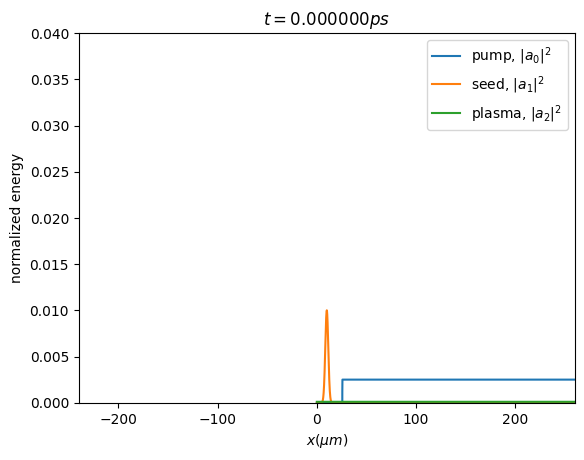
\includegraphics[width=\textwidth]{img/waves_t=0.png}
            \caption{Before waves interact.}    
        \end{subfigure}
        \begin{subfigure}[b]{0.5\textwidth}
            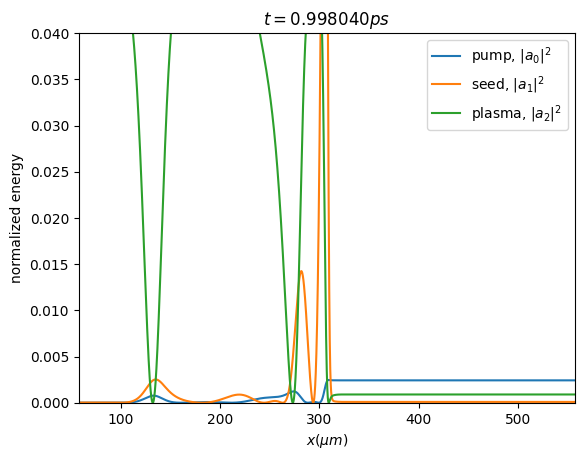
\includegraphics[width=\textwidth]{img/waves_t=1.png}
            \caption{Energy of pump is transfer to seed.}    
        \end{subfigure}
    \end{figure}

    \section{Conclusion}
    By sending a short laser pulse (seed) to a plasma with a counter-propagating pump laser, we observed the amplification of the short laser from numerical experiment. The energy is transferred from the pump wave to the seed wave. 

    \nocite{*}
    \bibliography{references}
    \bibliographystyle{plain}
\end{document}